\chapter{Разработка внутренних систем}
\label{cha:ch_2}
\section{Реализация вспомогательных систем}
Все вспомогательные системы спроектированы по паттерну ``Одиночка'' (Singleton) для \textit{Unity}, что означает, что на сцене и в ссылках на экземпляры класса компонента будет находиться только одна инициализированная на сцене сущность.

\subsection{Реализация spider-программы для сбора данных с GitHub.com}

\subsection{Реализация синглтона для объектов сцены}
Подробное описание основного функционала данного шаблона представлено в листинге \ref{monoSingleton}. Если описывать в двух словах реализацию этого довольно простого паттерна, то поведение наследников данного класса сводится к тому, что если при вызове поля Instance на сцене не окажется уже установленного объекта, то он создается и конфигурируется автоматически.

\begin{figure}[h]
	\centering
	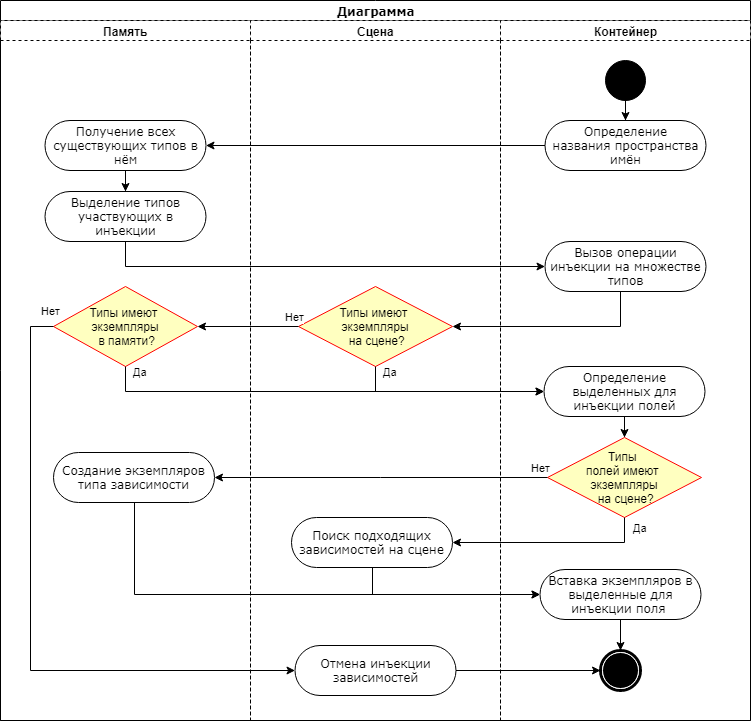
\includegraphics[width=\linewidth]{containerDI.png}
	\caption{Диаграмма деятельности работы DI контейнера для \textit{Unity}}
	\label{injectionIllustration}
\end{figure}

\subsection{Реализация DI контейнера для объектов сцены}
В качестве основного функционала контейнера представлен метод, который осуществляет проверку на участие в инъекции зависимостей, поиск подходящей зависимости и непосредственно инъекцию. Все три этапа работают по известному механизму описанному в стандарте JSR-299 \cite{jsr}, а именно: с помощью атрибутов, которые выполняют роль аннотаций, помечаются классы, участвующие в инъекции и поля, в которые нужно её проводить, далее контейнер на этапе запуска проекта проводит все инъекции. Бизнес-логика данного метода подробно представлена в листинге \ref{injectType}.

Для того чтобы провести инъекцию в целом продукте, также был реализован механизм, который вызывает вышеупомянутый метод на каждом найденном по названию пространства имен типе. Инъекция происходит в двух случаях: объекта из сцены в объект на сцене и объекта из памяти в объект на сцене. 

Данный принцип сюръекции нужен только для того, чтобы предупреждать появления ошибок при использовании или дополнении данного контейнера, когда объект, куда происходит инъекция, не создан на сцене или не инициализирован в памяти. Работа контейнера кратко описана в диаграмме деятельности на рис. \ref{injectionIllustration}.

\section{Создание базовой системы интеграции}
\subsection{Реализация базового инициализатора}
Для легкой интеграции данного продукта был реализован префаб пустого экземпляра класса GameObject, композиция которого содержит в себе единственный компонент (см. листинг \ref{initializer}) -- его работа  иллюстрируется алгоритмом \ref{alg:initializer}.

Механизм работы заключается в следующем: каждая из систем наследуется от интерфейса, который используется в зависимых классах и куда происходит инъекция. Сделано это было с требованием последнего принципа SOLID. Данный интерфейс также наследуется от другого интерфейса IATFInitializable, который содержит в себе единственный метод, отвечающий за инициализацию всех параметров системы после её создания на сцене путем вызова поля Instance. Далее происходит инициализация DI контейнера, настройка его на инъекцию в пространство имён ATF и вызов самой инъекции.

\subsection{Реализация расширенного инициализатора}
Описание атрибутного инициализатора

\subsection{Реализация адаптера для класса Input}
Далее представлен алгоритм \ref{alg:input}, составляющий бизнес-процесс класса адаптера, в котором и осуществляется перехват и вычисление относительно текущего состояния систем управления записью и хранилища (см. листинг \ref{input}). Кратко описывая принцип работы, можно выделить три ключевых метода: $Intercept, GetCurrentFakeInput, RealOrFakeInputOrRecord$. Они вызываются стеком, начиная с первого метода. 

Первым делом осуществляется перехват (в данном примере) входных данных Input.anyKeyDown, затем происходит вычисление записанного результата из STORAGE с помощью метода $GetCurrentFakeInput$, независимо от того, записывается ли процесс или проигрывается. Далее происходит решение, что выдавать на выход функции anyKeyDown в зависимости от того, в каком сейчас состоянии проигрыватель. Если происходит проигрывание, то выдается результат, который был сохранен в хранилище, если же происходит запись, то выдается результат Input.anyKeyDown и он же записывается в хранилище, а если ничего не происходит, то просто выдается результат, как если бы прослойки для записи вообще не существовало.

\subsection{Реализация расширенного модуля ввода}
Этот пользовательский модуль (см. листинг \ref{inputModule}) был спроектирован с целью дальнейшего расширения функционала по перехвату на внутреннюю систему обмена сообщениями внутри \textit{Unity}. Можно заметить, где конкретно реализован шаблон проектирования Bridge -- внутри StandaloneInputModule уже созданы события и описания поведения для работы с сообщениями ввода с периферийных устройств. Именно эти события и будут в будущем подвержены перехвату.

\section{Реализация основных систем}
\subsection{Реализация системы записи и проигрывания}
За основу системы записи и проигрывания был взят интерфейс (cм. листинг \ref{iRecorder}), регламентирующий поведение, схожее с недетерминированным автоматом, структура которого напоминает полный граф. Дело в том, что данная система подразумевает, что может происходить запись только одной структуры, которая составляет из себя набор различных вводов, в одну единицу вызова.

То есть, для того чтобы начать запись, необходимо первым делом использовать статичные методы ATFInput, во-вторых вызвать метод SetCurrentRecordingName и далее уже вызвать один из методов, изменяющих состояние проигрывателя, в данном конкретном случае -- StartRecord. Реализация интерфейса основана на главном свойстве структуры данных ``Очередь'' -- когда происходит запись, то пара FakeInput и объект значения записывается в очередь которая распологается внутри системы хранилища. Там же, при проигрывании выполняется выгрузка данной очереди в отдельную переменную и при каждом вызове перехватываемого метода, просто происходит выдача того, что было первым в этой очереди и так, раз за разом, пока вся очередь не опустошится.

\subsection{Реализация системы хранилища действий}
За основу поведения системы хранилища действий был взят интерфейс IATFActionStorage (см. листинг \ref{iStorage}), регламентирующий поведение книжной полки (статичного хранилища данных).

Принцип работы довольно прост, реализация данного хранилища базируется на вложенной структуре данных ``Словарь'' или иногда его называют хеш-таблицей. Внутри системы находятся поля следующих типов:
\begin{itemize}
	\item 
	\begin{verbatim}
	Dictionary<string, Dictionary<FakeInput, 
		Dictionary<object, Queue<Action>>>>;
	\end{verbatim}
	\item 
	\begin{verbatim}
	Dictionary<FakeInput, Dictionary<object, 
		Queue<Action>>>.
	\end{verbatim}
\end{itemize}

Первый тип -- это основное хранилище, туда происходит загрузка свежезаписанных сценариев, а также из жесткой памяти, например, из реестра. Второй тип -- это та самая переменная, в которую копируется очередь определенного типа ввода и которая опустошается на протяжении каждого перехватываемого вызова проверки ввода. Другие же методы отвечают за операции управления над самим хранилищем.

\subsection{Решение оптимизационной задачи системы хранилища действий}

\subsection{Реализация системы сохранения и загрузки хранилища действий}
Система сохранения и загрузки является PAC компонентом, она используется напрямую только хранилищем записанных действий. Интерфейс IATFActionStorageSaver (см. листинг \ref{iSaver}) отвечает за реализацию системы сохранения и загрузки хранилища в потенциально любой носитель информации.

Реализация интерфейса (см. листинг \ref{iSaver}) основана на работе с реестром через встроенный в стандартную библиотеку \textit{Unity} класс PlayerPrefs, обычно отвечающий за сохранение небольшой по количеству информации. Для сохранения сложных объектов эта реализация использует сериализацию в JSON объект всего хранилища либо же только одной записи, в зависимости от метода, который вызывается. Поведение реализации похоже на поведение недетерминированного автомата, по уже вышеупомянутым причинам.

\subsection{Реализация системы интеграции в готовую кодовую базу}

\subsection{Реализация системы упаковки данных хранилища}